\chapter{Anexos}

\section{Anexo Estimación de Casos de Uso}

\section{Anexos de Recopilación de Información}
Para la recopilación de información de este proyecto, se realizaron varias reuniones en modalidad remota con la administración de RVA. En las 3 reuniones realizadas, se le hicieron preguntas a la administración tanto para conocer su opinión acerca de la facilidad de uso del software que estaba en desarrollo, como para que tuvieran la oportunidad de sugerir cambios o mejoras de interfaz o usabilidad del sitio.

Además de las reuniones por llamada, también se creó un chat de texto en línea con los administradores, organizadores y moderadores que contaban con el tiempo para poder participar de el. En este chat, continuarían entregando sus opiniones a lo largo del desarrollo del software propuesto, mientras que también se les mostraban avances del proyecto.

\section{Anexo Aspectos de Gestión de Proyectos}

\subsection{Anexo Carta Gantt}

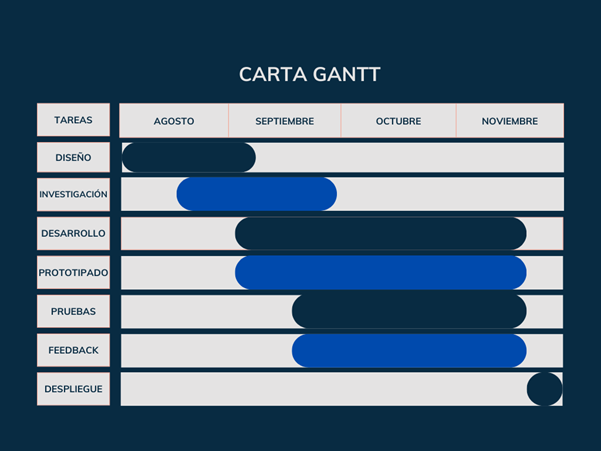
\includegraphics{gantt.png}

\subsection{Anexo Resumen de Esfuerzo}
\begin{center}
  \begin{tabular}{ | p{10cm} | p{5cm} |}
    \hline
    \multicolumn{1}{|c|}{\textbf{Actividad}} & \multicolumn{1}{|c|}{\textbf{Número de Horas}} \\
    \hline
    
    {Preparación del proyecto} & {20} \\ \hline
    {Desarrollo del módulo de autos} & {50} \\ \hline
    {Desarrollo del módulo de pistas} & {50} \\ \hline
    {Desarrollo del módulo de sesiones} & {80} \\ \hline
    {Desarrollo del módulo de temporadas} & {80} \\ \hline
    {Corrección de errores de código} & {40} \\ \hline
    {Despliegue de la aplicación} & {27} \\ \hline
    {Control de versiones} & {37} \\ \hline
    
    {\textbf{Total}} & {\textbf{384}} \\

    \hline
  \end{tabular}
\end{center}

\newpage

\section{Anexos Retrospectiva del Proyecto}

\subsection{Anexo Iteraciones en el Desarrollo}

\begin{center}
  \begin{tabular}{ | p{6cm} | p{3cm} | p {6cm} |}
    \hline
    \multicolumn{1}{|c|}{\textbf{Funcionalidad}} & \multicolumn{1}{|c|}{\textbf{Fecha}} &
    \multicolumn{1}{|c|}{\textbf{Retroalimentación}} \\
    \hline
    
    {Módulo de Autos (1)} & {12/11/2023} & {Añadir visualización para todos los autos y un sólo auto.}\\
    {Módulo de Autos (2)} & {12/11/2023} & {Agregar los autos tanto a la navegación como a la sub-navegación de la aplicación}\\
    {Módulo de Autos (3)} & {21/11/2023} & {Corregir problemas internos del modelo de autos}\\ \hline
   
    {Módulo de Pistas (1)} & {11/11/2023} & {Corregir problemas de validación en el modelo de Pista}\\
    {Módulo de Pistas (2)} & {12/11/2023} & {Agregaron las pistas tanto a la navegación como a la sub-navegación de la aplicación}\\
    {Módulo de Pistas (3)} & {28/11/2023} & {Mejorar la relación a modelos de Pista desde la visualización del modelo de Sesión.}\\ \hline
    
    {Módulo de Temporadas (1)} & {19/11/2023} & {Generar modelos de Ranking asociados a la temporada automáticamente después de crearla}\\
    {Módulo de Temporadas (2)} & {30/11/2023} & {Eliminar entradas de resultado de jugador asociadas a la temporada si estas tienen todos sus parámetros en cero}\\
    
    {Módulo de Sesiones (1)} & {19/11/2023} & {Determinar el número de cada sesión automáticamente una vez creada}\\
    {Módulo de Sesiones (2)} & {28/11/2023} & {Añadir botón de descarga para el Session Log asociado a cada sesión}\\
    {Módulo de Sesiones (3)} & {29/11/2023} & {Añadir acciones de administrador a la vista de sesión, tales como eliminar}\\
    
    \hline
  \end{tabular}
\end{center}
